\documentclass[onecolumn, draftclsnofoot,10pt, compsoc]{IEEEtran}
\usepackage{graphicx}
\usepackage{url}
\usepackage{svg}
\usepackage{setspace}
\usepackage{float}
\usepackage{longtable}
\usepackage{pgfgantt}
\usepackage{minted}
\usepackage{geometry}
\geometry{textheight=9.5in, textwidth=7in}


\def \subparagraph {.}

\usepackage{titlesec}
\usepackage{hyperref}

\titleclass{\threesection}{straight}[\subsection]
\titleclass{\foursection}{straight}[\subsection]

\newcounter{threesection}[subsubsection]
\newcounter{foursection}[threesection]

\renewcommand\thethreesection{\thesubsubsection.\arabic{threesection}}
\renewcommand\thefoursection{\thethreesection.\arabic{foursection}}

\renewcommand\theparagraph{\thethreesection.\arabic{paragraph}}
\renewcommand\theparagraph{\thefoursection.\arabic{paragraph}}

\titleformat{\threesection}
  {\normalfont\normalsize\bfseries}{\thethreesection}{1em}{}
\titlespacing*{\threesection}
{0pt}{3.25ex plus 1ex minus .2ex}{1.5ex plus .2ex}

\titleformat{\foursection}
  {\normalfont\normalsize\bfseries}{\thefoursection}{1em}{}
\titlespacing*{\foursection}
{0pt}{3.25ex plus 1ex minus .2ex}{1.5ex plus .2ex}


\makeatletter
\renewcommand\paragraph{\@startsection{paragraph}{6}{\z@}%
  {3.25ex \@plus1ex \@minus.2ex}%
  {-1em}%
  {\normalfont\normalsize\bfseries}}
\renewcommand\subparagraph{\@startsection{subparagraph}{7}{\parindent}%
  {3.25ex \@plus1ex \@minus .2ex}%
  {-1em}%
  {\normalfont\normalsize\bfseries}}
\def\toclevel@threesection{4}
\def\toclevel@foursection{5}
\def\toclevel@paragraph{6}
\def\toclevel@paragraph{7}
\def\l@threesection{\@dottedtocline{4}{7em}{4em}}
\def\l@foursection{\@dottedtocline{5}{10em}{5em}}
\def\l@paragraph{\@dottedtocline{6}{14em}{6em}}
\def\l@subparagraph{\@dottedtocline{7}{19em}{7em}}
\makeatother

\setcounter{secnumdepth}{4}
\setcounter{tocdepth}{4}
\setcounter{secnumdepth}{5}
\setcounter{tocdepth}{5}


% 1. Fill in these details
\def \CapstoneTeamName{			PolyVox}
\def \CapstoneTeamNumber{		66}
\def \GroupMemberOne{			Chris Bakkom}
\def \GroupMemberTwo{			Richard Cunard}
\def \GroupMemberThree{			Braxton Cuneo}
\def \CapstoneProjectName{		3D Virtual Reality Painting}
\def \CapstoneSponsorCompany{		EECS}
\def \CapstoneSponsorPersonOne{		Dr. Kirsten Winters}
\def \CapstoneSponsorPersonTwo{		Dr. Mike Bailey}

% 2. Uncomment the appropriate line below so that the document type works
\def \DocType{		%Problem Statement
				%Requirements Document
				%Technology Review
				Software Design Description (Draft 1/5/2018)
				%Progress Report
				}
			
\newcommand{\NameSigPair}[1]{\par
\makebox[2.75in][r]{#1} \hfil 	\makebox[3.25in]{\makebox[2.25in]{\hrulefill} \hfill		\makebox[.75in]{\hrulefill}}
\par\vspace{-12pt} \textit{\tiny\noindent
\makebox[2.75in]{} \hfil		\makebox[3.25in]{\makebox[2.25in][r]{Signature} \hfill	\makebox[.75in][r]{Date}}}}
% 3. If the document is not to be signed, uncomment the RENEWcommand below
%\renewcommand{\NameSigPair}[1]{#1}

%%%%%%%%%%%%%%%%%%%%%%%%%%%%%%%%%%%%%%%
\begin{document}
\begin{titlepage}
    \pagenumbering{gobble}
    \begin{singlespace}
    	
\includegraphics[height=4cm]{coe_v_spot1}
        \hfill 
        % 4. If you have a logo, use this includegraphics command to put it on the coversheet.
        %\includegraphics[height=4cm]{CompanyLogo}   
        \par\vspace{.2in}
        \centering
        \scshape{
            \huge CS Capstone \DocType \par
            {\large\today}\par
            \vspace{.5in}
            \textbf{\Huge\CapstoneProjectName}\par
            \vfill
            {\large Prepared for}\par
            \Huge \CapstoneSponsorCompany\par
            \vspace{5pt}
            {\Large\NameSigPair{\CapstoneSponsorPersonOne}\par}
	    {\Large\NameSigPair{\CapstoneSponsorPersonTwo}\par}
            {\large Prepared by }\par
            Group\CapstoneTeamNumber\par
            % 5. comment out the line below this one if you do not wish to name your team
            \CapstoneTeamName\par 
            \vspace{5pt}
            {\Large
                \NameSigPair{\GroupMemberOne}\par
                \NameSigPair{\GroupMemberTwo}\par
                \NameSigPair{\GroupMemberThree}\par
            }
            \vspace{20pt}
        }
        \begin{abstract}
        % 6. Fill in your abstract    
At this point in the term, team PolyVox has constructed a functional alpha build of each of the primary elements of the program. A basic user interface has been designed and built, a functioning voxel engine has been constructed, and the graphics engine has successfully compiled. At this point the team is focusing their efforts on combining their sections into a unified system, and to begin work towards a feature complete beta build.
        \end{abstract}     
    \end{singlespace}
\end{titlepage}
\newpage
\pagenumbering{arabic}
\tableofcontents
% 7. uncomment this (if applicable). Consider adding a page break.
%\listoffigures
%\listoftables
\clearpage

% 8. now you write!

\subsection{References}
\bibliographystyle{IEEEtran}
\bibliography{Bibliography}{}

\section{Introduction}
The long term goal of the project is to create a robust and user-extensible 3D art program for virtual reality. To that end, the project has been divided into three primary sections, a dedicated front, middle and back end, with each assigned to a team member. The front end entails the user interface and compatibility with the VR hardware. The middle end acts as an intermediary between the front and back end, taking user input and relaying it as commands to the back end. The back end acts as the graphics engine underpinning the program. At this point in the project, the PolyVox team has developed a alpha build of each of the primary components. The front end is semi-functional with a prototype interface designed. The middle end acts as a working voxel engine, calling the native rendering software from unity. Finally, the back end’s graphics engine has successfully compiled and is capable of basic input and output.

The current goals of the project are based around integrating the disparate elements of the project into a single working system. Each section currently operates independently, with the front and middle ends calling dummy functions, and with the back end only operating with basic functionality. The team will begin merging these elements in the coming weeks, with front and middle end integration being the first step. Following that, the middle end will begin implementing calls to the back end API, replacing existing calls to the unity graphics engine. The back end will continue with its its development cycle, adding additional functionality over time.

\section{Chris Bakkom}
\subsection{Alpha Goals}
The purpose of this alpha is to create a structure for implementing our feature set. This alpha build will be attempting to prove the feature availability that we have to create a platform for integrating our tools. In terms of the UI layer, this means getting a working structure for the tool-belt and the buttons and functions that each tool can contain. This will require 3D objects to be displayed for the user and require them to be intractable by user input. There also needs to be a way to capture the input from the VR devices so we have a way of taking our VR inputs and registering them to our system.

\subsection{Progress}
The structure of the 3D UI has been completed. Each of the 3D blocks on the tool belt can be accessed through user input. Right now they can be accessed through keyboard shortcuts. Each block has the space for any UI element, with the potential to interact with other scripts in the program. The test that has been run for this is the middle UI block set up, with button states to run test scripts. These scripts have arbitrary properties like changing other objects in the scene or running arbitrary scripts. However, this is proof that the UI layer can effectively interact with all other top layer functions in the program. The UI manager captures all states and input from the UI and can manipulate scripts further down in the pipeline. This will be important when integrating the future tools and functionality that will need to be compatible with the UI. 
The UI has been broken down in the following abstraction. The UI Blocks are at the top level where they are comprised with accessor scripts that modify their state and position. Each block is fixed in relative view of the display. This means that wherever the user is looking, the blocks will be in that same position. If we did not like the look of the tool belt, we could move the blocks to another location and they would still track alongside the display. Each block has two states, selected and non-selected. The non selected state simply places them in a predetermined location and gives them some transparency. This will allow the UI to have an inactive state where we can specify how much we want to display to the user in this mode. In coordination with the client, we can determine if the transparency is enough to refute the inactive UI as a non-distraction, or we can remove it from the view entirely. The selected state turns up the transparency and invokes the 2D UI that the block has access to. This allows us to create custom UI panes for each block. Each block can now have separate panes and functions that are specific to the tool. This is not only important for separating all of the custom functionality, but it also provides a framework for allowing future renditions. From there, each 2D UI can have any number of buttons, toggles, sliders and states for defining the tools purpose. This will allow for any kind of functionality we want to implement into our beta in coordination with the interchange layer.
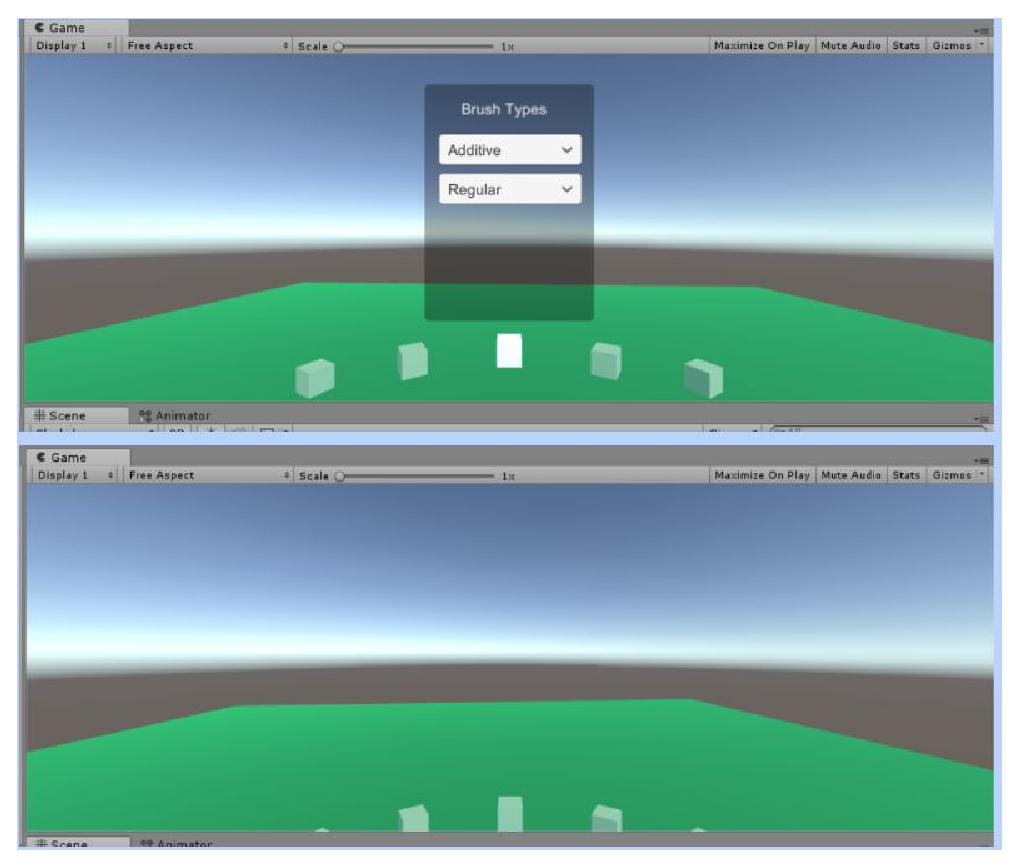
\includegraphics{image1}

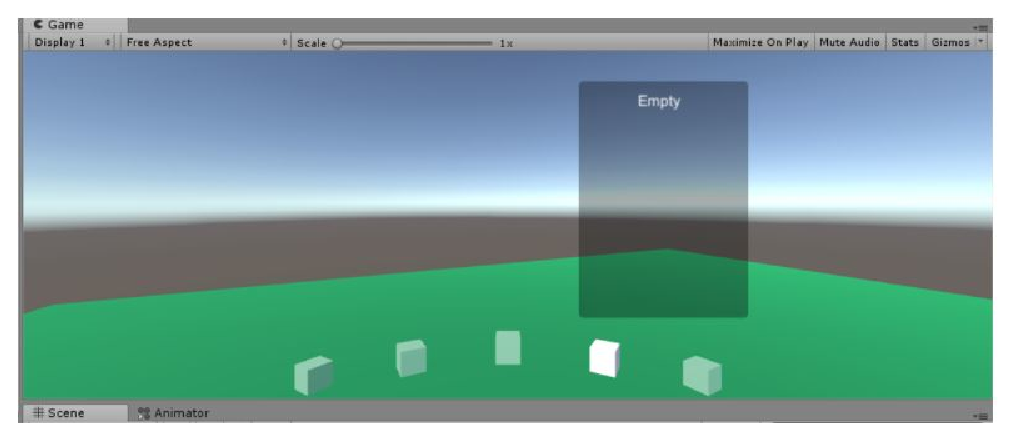
\includegraphics{image2}
\subsection{Left for Beta}
The UI functions needs to be accessible through VR inputs. This means taking the VR controller inputs and mapping them to UI interactions. The entire UI needs to be accessed through the VR interface, so each function in the UI will have an onto mapping from the VR controllers. The captured button presses and touchpad movements will grant this access. 
All of the features we want for beta must be accessible through the UI. This means creating all the buttons, toggles and settings we need through the UI prototype. This also means we need to map each of the buttons and states to their corresponding interchange functions. Each of the available functions in the interchange will have a mapped script from the UI layer. Right now there are five blocks for prototyping the tools we want to include into beta. This number can change depending on how much we want to include. Since each UI block has its own custom UI script, the first priority will be to include the feature complete prototypes. The brush colors, brush styles, saving and loading states are the minimum for a feature complete beta. Each of these already has a dedicated UI block, but the custom scripts still need to be implemented. This means creating all of the details between each of these functions. The save tool will need a path and an action for saving. The Load tool will need a path and an action for loading. The brush color will need a custom color picker. The brush style will need a weight slider and a drop down for switching between additive and subtractive states. This will encompass everything we need for a feature complete beta in terms of our UI functionality. 
The last thing that we would like for beta is animation for the UI. Right now, the switches between an active and inactive UI are hard switch states. This might be slightly jarring for the user, so as an added bonus, the UI will have some subtle animations for switching between these states. 

\subsection{Problems and Solutions}
The biggest problem with the top level layer of the program is access to hardware. Right now we are using the VR lab on campus. This has worked for prototyping our program to gather some of the basic functionality that is required. However, when building our beta we will need to have full access to development tools. The on-campus resources are limited so development time is scarce. To solve this, we will need our own hardware to develop on. This means acquiring our own HMD and Controllers as well as a dedicated VR machine. The biggest blocker for having a VR compatible machine is the high end graphics card required for running the HMD output. This will be the highest priority in our development pipeline. 

\section{Richard Cunard}
\subsection{Purpose}
The middle-end of the program is meant to receive user input from the VR and motion control interface, process the input into commands, and translate those into instructions for the Yggdrasil engine, as well as provide high level management of memory allocation and a hierarchy of spatial subdivisions (known as blocks) to Yggdrasil. At this point in the project, however, Yggdrasil is still under construction, and is currently unable to display geometry to the degree needed for basic functionality. As such, the alpha build of the front and middle end use the Unity engine’s native graphics engine for rendering, and is able to function independently from VR input, acting completely on its own for testing purposes.

\subsection{Current State}
Currently, the voxel engine is capable of creating, destroying, and changing the color of existing voxels. Additionally, as a minor stretch goal for the alpha build, the system is capable of adjusting the ‘brush weight’ of the cursor, increasing or decreasing the number of voxels created at a time, increasing and decreasing in cubic increments as directed by the user. In the current build, which does not yet integrate the motion control interface, the inputs are performed using a keyboard, which controls a cursor meant to represent the user’s ‘brush’. Blocks are placed at the point the cursor is located at any given moment.

As of yet, the main features left to complete include the saving and loading of a voxel state, as well as the integration of VR and motion control compatibility. This is, of course, not including the implementation of the Yggdrasil graphics engine, which is meant to make the program much more powerful and efficient. The implementation of a save/load feature in the program’s current state would be relatively trivial to implement, however, the team may choose to wait, instead implementing a dummy save feature, until Yggdrasil is integrated, as doing so will effectively invalidate any save/load system put into place. Finally, memory management and block hierarchy have yet to be implemented, though the latter is nearly complete on its own.

\subsection{Next Steps}
Once Yggdrasil is in a development-ready state, the next step will to begin implementing its API into the existing structure within the alpha build. This will mean replacing calls to Unity’s rendering system with calls for memory reservation and code injection within Yggdrasil. This will mean totally reconstructing the functions that the current implementation calls. However, the current build was designed with this in mind, with functions concerning rendering and voxel manipulation able to be slotted in and out as needed. This will, hopefully, allow for a smooth transition when implementing Yggdrasil.

\subsection{Challenges}
The primary challenge thus far has been developing the system without the graphical back-end completed. As much of the middle-end functionality is functionally dependent on having Yggdrasil, it has become necessary to assemble a significant amount of prototype code that will be disposed of in the future. In order to salvage some of these efforts, the current iteration of code is written in such a way as to be able to replace existing function calls and replace them with ones that will reference the Yggdrasil API at a later date. As of yet, only four colors of voxel can be created, as the system relies entirely on static textures for its coloration. However, this is easily extensible, with future versions being planned to allow for full color selection using the system renderer. 

\subsection{Functionality}
The code itself uses a series of techniques common to voxel-based applications. Voxels are stored in a three-dimensional integer array, in which each element corresponds to a coordinate that may or may not contain a voxel. Each voxel face is made from two triangles, generated via a function which is fed a point, and creates a set of vertices relative to that point, the basis of the voxel’s geometry. From there, the triangles generated are fed to a unity function which renders them.

\begin{minted}
[
frame=lines,
framesep=2mm,
baselinestretch=1.2,
linenos
]{C}
void CubeBack(int x, int y, int z, int block)
    {
        tempVerts.Add(new Vector3(x, y - 1, z));
        tempVerts.Add(new Vector3(x, y, z));
        tempVerts.Add(new Vector3(x + 1, y, z));
        tempVerts.Add(new Vector3(x + 1, y - 1, z));

        Vector2 color = new Vector2(0, 0);

        if (Block(x, y, z) == 1)
        {
            color = blue;
        }
        else if (Block(x, y, z) == 2)
        {
            color = green;
        }
        else if (Block(x, y, z) == 3)
        {
            color = red;
        }
        else if (Block(x, y, z) == 4)
        {
            color = yellow;
        }

        Cube(color);

    }
\end{minted}
When a voxel is generated, a function determines which faces are exposed to the user. Sides not exposed are not rendered. Voxels are changed using a set of functions that are called on user input (currently in the form of a keyboard button.) Each of these functions changes one or more elements of the array that maps the scene, with zero corresponding to and empty space, and 1 through 4 corresponding to a blue, red, green or yellow block respectively. Once the state is called, the scene is redrawn with the change of state implemented. 
\begin{minted}
[
frame=lines,
framesep=2mm,
baselinestretch=1.2,
linenos
]{C}
//check for user input
	void Update ()
    {
        //if input is received, check controller position and change voxel state at the controller coords
        if (Input.GetButton("Blue"))
        {
            changeState(controller.x, controller.y + 1, controller.z, 1, w);
        }

        else if (Input.GetButton("Green"))
        {
            changeState(controller.x, controller.y + 1, controller.z, 2, w);
        }

        else if (Input.GetButton("Red"))
        {
            changeState(controller.x, controller.y + 1, controller.z, 3, w);
        }

        else if (Input.GetButton("Yellow"))
        {
            changeState(controller.x, controller.y + 1, controller.z, 4, w);
        }

        else if (Input.GetButton("Destroy"))
        {
            changeState(controller.x, controller.y + 1, controller.z, 0, w);
        }

        else if (Input.GetButtonDown("WeightUp"))
        {
            w++;
            Debug.Log("WeightUp");
        }

        else if (Input.GetButtonDown("WeightDown"))
        {
            if (w != 1)
                w--;
        }

        //reload current chunks
        LoadChunks(GameObject.FindGameObjectWithTag("Player").transform.position, 200, 300);
    }
\end{minted}
Finally, the system works by chunking, a process by which sections of the scene are loaded and unloaded from the application to conserve memory. Which chunks are loaded corresponds to the position of the camera, with chunks loading in as the camera becomes closer and loading out as the camera moves away.
\begin{minted}
[
frame=lines,
framesep=2mm,
baselinestretch=1.2,
linenos
]{C}
public void GenerateMesh()
    {

        for (int x = 0; x < chunkSize; x++)
        {
            for (int y = 0; y < chunkSize; y++)
            {
                for (int z = 0; z < chunkSize; z++)
                {
                    //This code will run for every block in the chunk

                    if (Block(x, y, z) != 0)
                    {
                        //If the block is solid

                        if (Block(x, y + 1, z) == 0)
                        {
                            //Block above is air
                            CubeTop(x, y, z, 0);
                        }

                        if (Block(x, y - 1, z) == 0)
                        {
                            //Block below is air
                            CubeBot(x, y, z, Block(x, y, z));

                        }

                        if (Block(x + 1, y, z) == 0)
                        {
                            //Block east is air
                            CubeRight(x, y, z, Block(x, y, z));

                        }

                        if (Block(x - 1, y, z) == 0)
                        {
                            //Block west is air
                            CubeLeft(x, y, z, Block(x, y, z));

                        }

                        if (Block(x, y, z + 1) == 0)
                        {
                            //Block north is air
                            CubeFront(x, y, z, Block(x, y, z));

                        }

                        if (Block(x, y, z - 1) == 0)
                        {
                            //Block south is air
                            CubeBack(x, y, z, Block(x, y, z));

                        }

                    }

                }
            }
        }

        UpdateMesh();
    }
\end{minted}


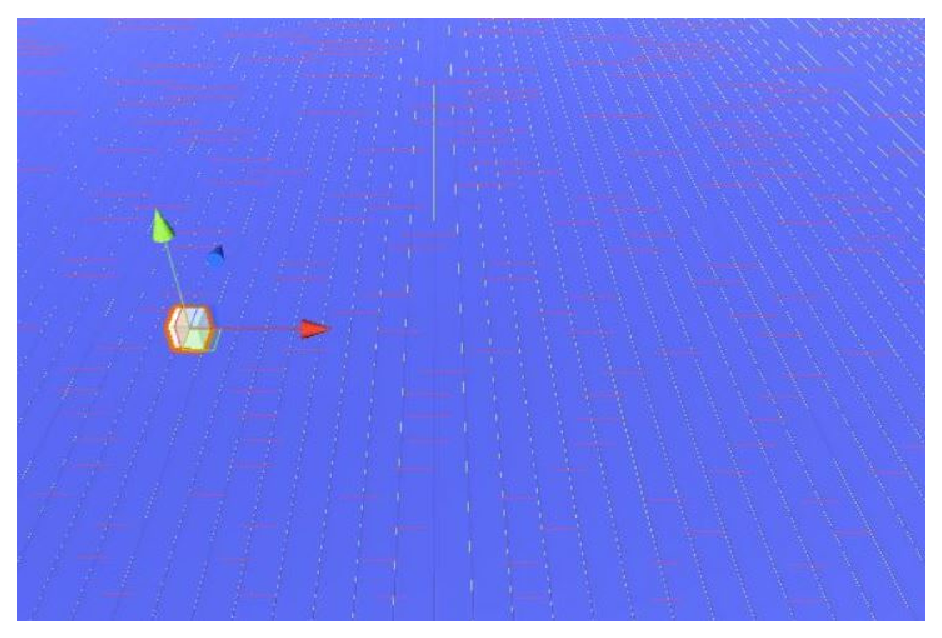
\includegraphics{image3}

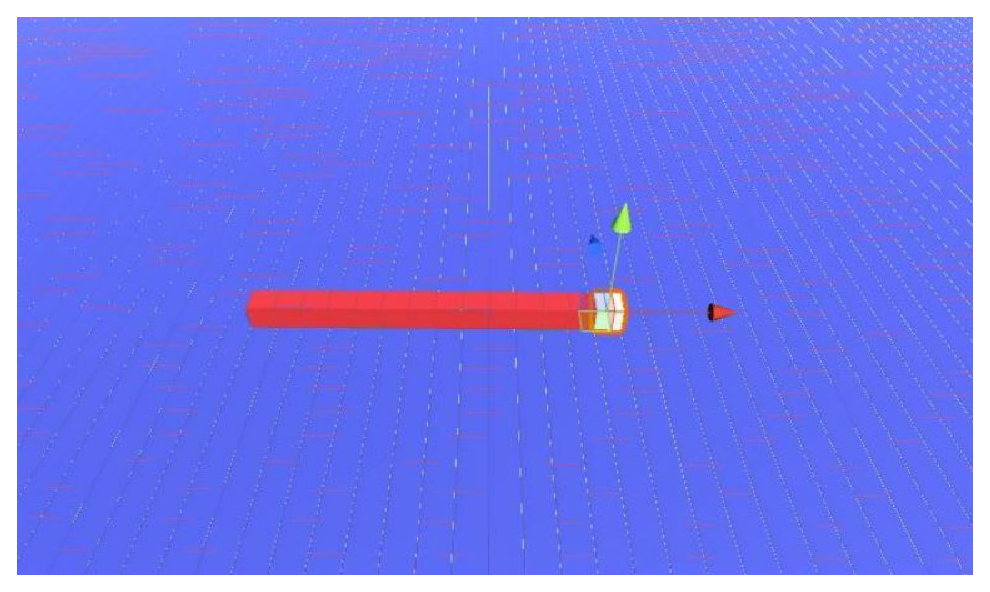
\includegraphics{image4}

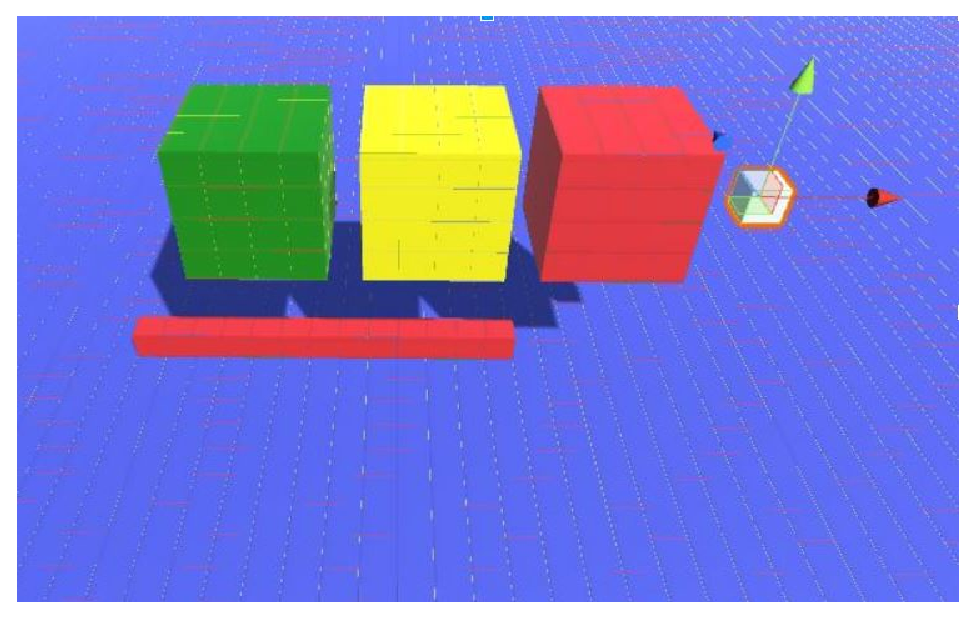
\includegraphics{image5}

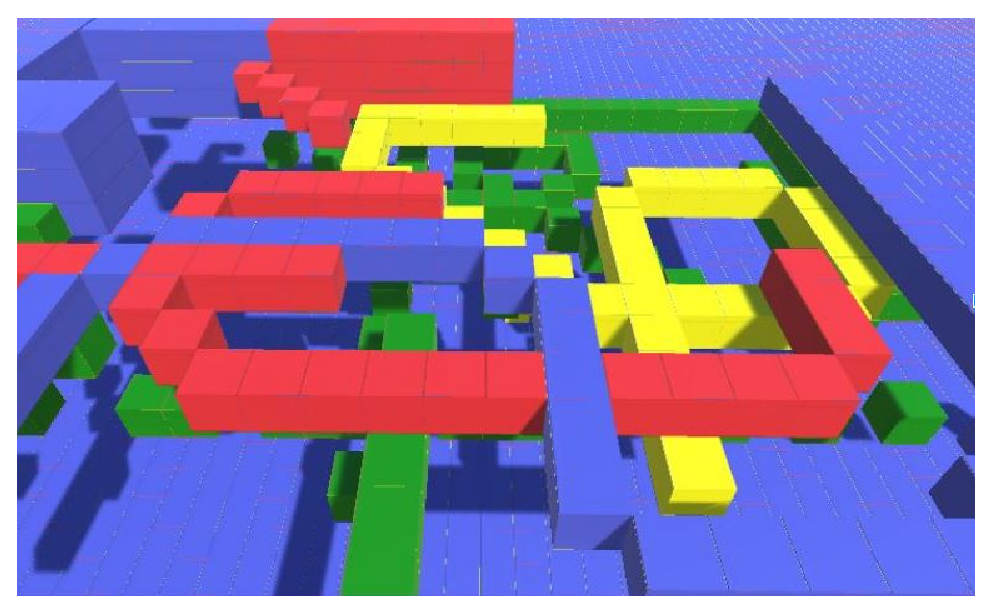
\includegraphics{image6}

\section{Braxton Cuneo}
The backend of PolyVox, as per the current state of the design document, is a set of GPGPU programs, dubbed “Yggdrasil”, which carry out the heavy lifting of managing, manipulating, and rendering the data backing the virtual environment represented by PolyVox. For the sake of proper context, below is a brief overview of the operation of Yggdrasil.

\subsection{Operation}
The state of Yggdrasil, between the execution of its constituent programs, consist of four buffers, called the Data Buffer, the Heap Buffer, the Block Buffer, and the Exchange Buffer.

The Data Buffer houses almost all of the data representing the content of the virtual environment, including all of the geometry which is contained within it. The Data Buffer also acts as a source of spare memory for allocation by threads in Yggdrasil programs. Regardless of application, the memory housed within the Data Buffer is always managed in sections of 64 bytes, with no unit of 64 bytes overlapping with any other unit. These units are known as “nodes”.

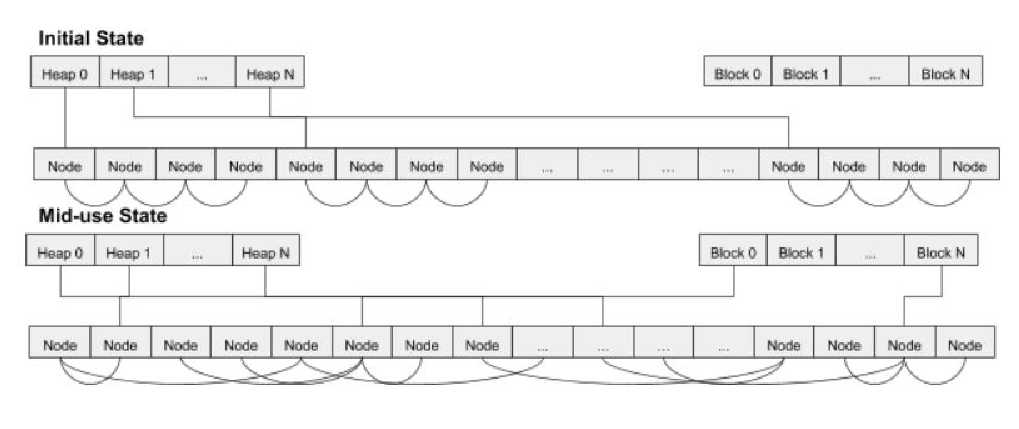
\includegraphics{image7}

Nodes that are not in use are distributed among a set of linked lists, the address of the head of each linked list is stored alongside the length of that linked list in pairs. Each of these pairs are, in turn, stored as elements in the Heap Buffer, which acts as a means for program threads to allocate and free nodes.

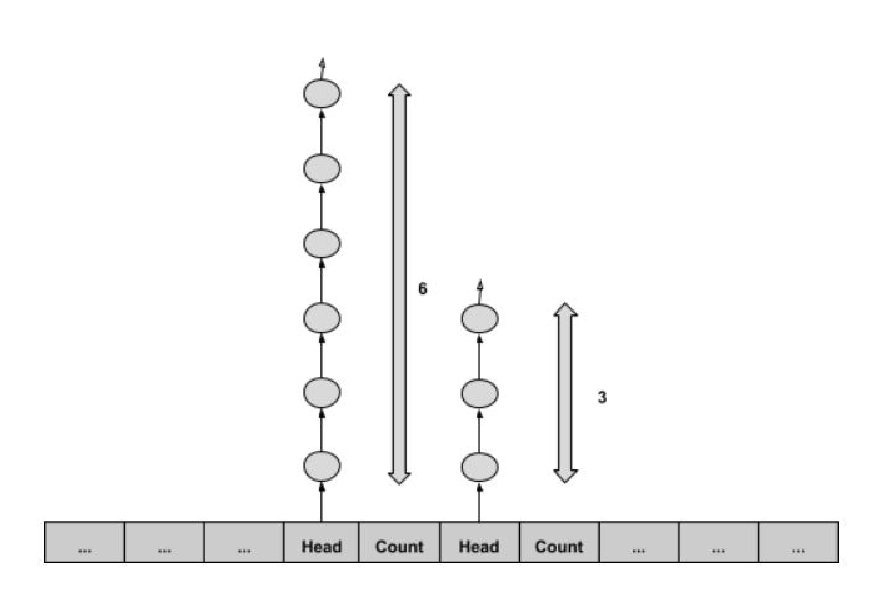
\includegraphics{image8}

Geometry is represented as voxels in a sparse voxel octree (SVO), and there can be more than one sparse voxel octree in a given scene. The contents of each SVO in the environment represented by PolyVox is mapped to the inside of a three-dimensional box with bounds described by a 4x4 transformation matrix, assuming that the pre-transform bounds of the box make up an axis-aligned cube of side length two centered at the origin. These boxes are known as “Blocks”. The address of the root voxel of a given block, as well the transformation of that block and some other key information, is stored as a struct in the Block Buffer, with each block having a unique address in the buffer.

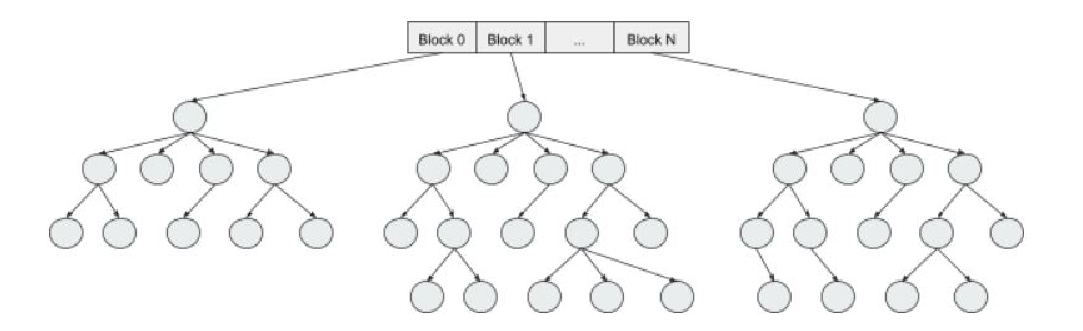
\includegraphics{image9}
In order to exchange data back and forth between the GPU and CPU in and efficient manner, it helps that the data comes pre-packed in its own space, apart from the memory space of the Data Buffer. This is why the Exchange Buffer exists.

In addition to these buffers, there is also the Task Buffer, which acts in a similar manner to the Heap Buffer, but it is used during program execution to distribute tasks among the threads of the running program.

To manage, render, and manipulate this state, Yggdrasil has a set of programs. The first of these is the Initializer, which clears the Task Buffer, breaks down the Data Buffer into a series of evenly sized linked lists and distributes the linked lists over the Heap Buffer. This sets up the state of the buffers such that all memory is accounted for and that there are no hanging references.

Another Yggdrasil program is the MemoryManager, which performs balancing operations over the Heap Buffer, evening out the lengths of each list.

The exchange of data between the GPU and CPU is performed by the Tree Manager, which is in charge of finding nodes to insert or cull from the state of PolyVox and performing the necessary data packing and unpacking on the GPU-side.

The RayTracer is the program in charge of rendering the scene. In essence, it performs a voxel cone trace operation starting at the corresponding location for each pixel in the output image and moving away from the position of the camera. In its most simple form, it simply traces at a depth in an SVO corresponding to its distance from the camera, with it traversing deeper in the SVO the closer it is. This is done until the trace reaches a certain level of opacity in its sample, at which point it returns its accumulated sample color to the pixel.

The Basic Brush Template is a template of compute shader code into which the interchange injects foreign shader code. The template handles all of the boilerplate operations involved with performing a brush operation onto the state of Yggdrasil, only calling the injected code at key parts of the operation, such as determining the color of a voxel.

\subsection{Problems and Progress}
Since the previously submitted progress report, the majority of the functionality of Yggdrasil was written into prototype GLSL code. This code was distributed among several files, one for each program and an additional one for commonly used functions. 

Unfortunately, once this code was incorporated into a Unity project to begin compilation checks and unit testing, it became evident, over several days of research, trial and error, that Unity does not support GLSL code in compute shaders. This lack of functionality is contrary to what Unity states in its published documentation, but nonetheless is apparent by the lack of any instance or example of GLSL-based Unity compute shaders available online and, furthermore, the unanswered support requests of several users with similar troubles over several years. Considering the potential wait times involved with getting a program such as Unity patched, if it is patched at all to enable GLSL compute shaders, it was deemed best to port the GLSL code to HLSL.\cite{unity}

After porting the code in question, the resulting HLSL code reached successful compilation within a few days, although with some caveats. Given the performance requirements of PolyVox, it was hoped that the program could take advantage of Unity’s Vulkan capabilities. Unfortunately, these capabilities are still experimental, and the automatic shader translation from HLSL to GLSL Unity performs for working with Vulkan creates code with syntax errors. Thus, for the sake of maintaining overall functionality, Unity’s Vulkan capabilities were excluded from the project’s building process.

Once the backend code was successfully compiled, several unit tests were created in order to ensure that the state of PolyVox was created correctly by Yggdrasil’s initialization program and that the code in charge of managing memory allocation and task scheduling operated correctly. This process encountered some difficulties, as Unity offered little documentation regarding the specifics of resource binding. Particularly, the published documentation failed to specify that structured read-write buffers, rather than standard read-write buffers, were the type of compute buffers that Unity binds by default. This resulted in some confusion, as this meant that the CPU-side program was not able to bind to the resources in Yggdrasil, so data supposedly fetched from the GPU-side state were simply zeroed buffers. Once this discrepancy was realized, it was resolved simply by changing the compute buffers used by Yggdrasil to structured read-write buffers.

In its current state, Yggdrasil has five programs, the Initializer, RayTracer, MemoryManager, TreeManager, and Diagnostic. Of these programs, all but TreeManager compiles, and those that do compile can reliably be executed as well as input and output through Unity. To give a general sense of how the compiling programs operate, below is the main function for each of these programs.

\subsection{Future Plans}
Whether or not programs compile has little bearing over whether perform as they should when executed. This is the task that still lays ahead in order to complete the backend. Verifying performance will be done through several stages, first testing the most basic functionalities of the programs and eventually testing the most high-level aspects of the programs. From there, the remaining programs that have yet to be rendered executable will be finished and then tested.

The first stage of testing will be verifying that the Initializer program correctly initializes the data buffer, memory buffer, and task buffer such that every node of memory in the data buffer is listed once and only once as free memory in the heap buffer’s heaps and that all task queues in the taks buffer are empty. This is crucial to confirm before further developing Yggdrasil because a flawed starting state will result in hanging references or memory leaks which can cause a great deal of erroneous operation.

Once the initializer is confirmed to be working properly, the Diagnostic program is used to confirm that both the memory management, task scheduling, and data structure functionalities of Yggdrasil work as per specification. Testing will be performed by repetitively allocating and freeing memory, grabbing and posting tasks, as well as pushing and popping from stack data structures in a manner that can be easily verified for correctness. Then, if the state of a thread is deemed to not match what it should, the details of what went wrong are reported to the CPU via the exchange buffer. These specific functionalities are in the second stage of testing because bugs in memory management or task scheduling systems, in addition to rendering the rest of Yggdrasil’s operation flawed, are very difficult to root out and can pervade all higher-level functionalities.

After confirming the proper operation of resource management, the MemoryManager and RayTracer programs are both subjected to testing. Both are as a basic matter of ensuring correct operation, however ensuring the proper operation of the RayTracer is of crucial importance, because it offers the best indication to developers that the system is working properly. Furthermore, having an operation RayTracer program makes the matter of developing the BasicBrush program template easier, which will help to ensure the full operation of Yggdrasil by the start of the expo.

Once all basic operations have been confirmed to work as per specification, the remainder of development will be devoted to refining the operation of Yggdrasil. This refinement will mainly consist of either adding additional features to the ray tracing or brush capabilities of the system or decreasing the computational or storage cost of using PolyVox. For instance, the RayTracer, in its current state, cannot ray trace through more than one block at a time meaning that the transparency that can be rendered through the system when there are multiple blocks on the screen may not be particularly consistent or realistic. There are already features listed in the specification (though not the requirements document) which can resolve this issue with transparency, but not without greatly increasing the complexity of ray tracing. Hence, these sorts of features are reserved for the latter portion of development as stretch goals.

\section{Conclusion}
In total, all three portions of PolyVox have experience appreciable progress. The front end, which is in charge of relaying motion and touch input from the user to the middle end and displaying imagery from the back end to the user, is already capable of giving the user a fluid view of a virtual environment as well as registering input from motion controls. The middle end, which is charged with interpreting events from the front end and executing programs from the back end in response, can already signal for the creation and destruction of blocks in a simulated back end. Lastly, the back end, which is meant to handle the heavy lifting of managing the data backing the virtual environment of PolyVox, as well as its rendering and manipulation, has most of its functionality written out as HLSL compute shaders.

With regards to the future of the project, the next steps to be taken for the front and the middle end are to begin developing and refining their interoperation, as they will need to communicate with one-another well to create a seamless experience for the user. Meanwhile, the code currently written for the back end must have its operation tested and verified and have the remainder of its functionality coded in prior to final incorporation with the middle and back ends.

\end{document}
